% !TEX root = ../thesis.tex
\chapter{Introduction}
\label{Introduction}
\thispagestyle{empty}


\section{Context}
Many technologists consider chatbots one of the hottest technologies in recent time (https://bit.ly/2od0Tdw), an opinion fueled for example by Facebook’s release of its Messenger API in 2016. In April 2017, Facebook reported 100,000 monthly active bots on the Messenger platform. In March 2017 Varol et al. \cite{Varol} estimated that between 9\% and 15\% of active Twitter accounts ar bots (29-49 million accounts out of 328 millions, https://bit.ly/2v3AT6O). Gartner estimates that by 2020 85\% of customer requests will be handled by bots, while Inbenta estimates 1.8 billion unique customer chatbot users by 2021 \cite{inbenta}.

The technological advancements of chatbots undoubtedly produced a hype on its own, yet bots today are by far not limited to instant messaging only. Bots permeate all kinds of on-line conversations in Twitter, Facebook, Instagram, Q\&A sites, on-line newspapers, emails, and the like. They are everywhere where there are humans conversing with each other via the Internet, legitimately or illegitimately. For example, Messenger explicitly allows bots in its chats, while WhatsApp states that it blocks phone numbers generating bot traffic (https://bit.ly/2HhW9wG).

Inspired by Bessi and Ferrara \cite{bessi}, we understand bots generically as algorithmically driven entities that on the surface act like legitimate human users in on-line conversations.

Daniel et al. \cite{DanielIC2019} has started asking the question whether this increasing presence of bots may lead to harmful communication patterns that may hurt the human participant in the conversation, and we found a variety of anecdotal evidence that this may indeed happen. Of course, bots are not harmful in general. But sometimes, intentionally or unintentionally, software-driven conversations may just break common conversational rules, etichette, or even law. It is important to acknowledge the problem, so as to be able to provide countermeasures and to prevent people from getting hurt.

A \textbf{harm} occurs when someone suffers an injury or a damage, but also when someone gets exposed to a potential adverse effect or danger. In a prior work \cite{DanielIC2019}, we identified examples for the following types of harm caused by bots:

\begin{itemize}
	\item[\PencilRight] \emph{Psychological harm} occurs when someone's psychological health or wellbeing gets endangered or injured; it includes feelings like worry, depression, embarrassment, shame, guilt, anger, loss of self-confidence, or inadequacy. An example of a bot causing psychological harm is Boost Juice's Messenger bot that was meant as a funny channel to obtain discounts by mimicking a dating game with fruits but used language that was not appropriate for children (\url{http://bit.ly/2zvNt0E}).
	
	\item[\PencilRight] \emph{Legal harm} occurs when someone becomes subject to law enforcement or prosecution; it includes for example the breach of a confidentiality agreement or contract, the release of protected information, or threatening. A good example is the case of Jeffry van der Goot, a Dutch developer, who had to shut down his Twitter bot, which generated random posts, after the bot sent out death threats to other users (\url{http://bit.ly/2Dfm71P}). 
	
	\item[\PencilRight] \emph{Economic harm} occurs when someone incurs in monetary cost or looses time that could have been spent differently, e.g., due to the need to pay a lawyer or to clean one's own social profile. A concrete example of an infiltration by a bot happened on Reddit in 2014, where the bot wise shibe provided automated answers and users rewarded the bot with tips in the digital currency dodgecoin, convinced they were tipping a real user (\url{http://bit.ly/2zu2b6r}).
	
	\item[\PencilRight] \emph{Social harm} occurs when someone's image or standing in a community gets affect-ed negatively, e.g., due to the publication of confidential and private information like a disease. An example of a bot causing social harm was documented by Jason Slotkin whose Twitter identity was cloned by a bot, confusing friends and followers (\url{http://bit.ly/2Dfq4DH}). 
	
	\item[\PencilRight] \emph{Democratic harm} occurs when democratic rules and principles are undermined and society as a whole suffers negative consequences, e.g., due to fake news or the spreading of misinformation. Bessi and Ferrara \cite{bessi}, for instance, showed that bots were pervasively present and active in the on-line political discussion about the 2016 U.S. Presidential election (predating Robert S. Mueller III's investigation into the so-called Russian meddling).
\end{itemize}

These types of harm may happen while bots perform  \textbf{actions}, such as posting a message or commenting a message by someone else, that are not harmful per se and that also human users would perform. What needs to happen is the verification of some condition of inappropriateness, which turns the action into an \textbf{abuse}. Abuses that can be found are, disclosing sensitive facts, denigrating, being grossly offensive, being indecent or obscene, be threatening, make false allegations, deceive users, spam, spread misinformation, mimic interest, clone profiles, and invade spaces that are not meant for bots \cite{DanielIC2019}. Some of these may be subject to legal prosecution (e.g., threatening people), others only breach moral, ethical or social norms, yet they still may be harmful to unprepared, human users.

\section{Problem Statement and Contributions}
\label{sec:contributions}
In this thesis, we focus on \textbf{Twitter} as online communication environment, as Twitter is freely accessible through its open API (\url{https://developer.twitter.com}) and does not require special friend privileges to access content of users. We specifically study content shared via \emph{tweets}, where a tweet $t$ is a short text message of up to 280 characters, including URLs to external content or images, mentions (annotated references of other Twitter accounts), and hashtags. We neglect direct messages (similar to chats) between users, as these are private and not available for inspection. 

\textbf{Bots} manifest themselves in Twitter as regular users: they have an own account and user profile and are able to tweet (post a message), re-tweet (forward a tweet), reply to tweets, like tweets. Through the API of Twitter, it is possible to retrieve all tweets of a given account, that is the tweet timeline of the account, for inspection. For the purpose of this thesis, we focus on the tweets produced (tweets, re-tweets, replies) and interpret a generic user as a tuple $u = \langle P, T \rangle$ where $P$ is the set of 
user profile parameters (e.g., name, bio, location) and $T = [t_i,...,t_n]$ is the chronologically ordered sequence of tweets.

Out of the different types of \textbf{abuses} listed above, in this thesis we concentrate on: \emph{Fake-Followers} that follow a user to pretend interest in the user; bots that spread \emph{adult content} like pornographic material or lures (Not Safe For Work); bots propagating news and potential \emph{misinformation}, i.e., high-frequency publishers of news of ambiguous quality; and \emph{Spam-Bots} distributing commercial advertisements. The selection of these four abuse types is motivated by the common method we propose for their analysis, i.e., feature-based classification.

If we call the four classes of bots \emph{NSFW, News-Spreaders, Spam-Bots, Fake-Followers}, respectively, 
and use the class \emph{Genuine} for genuine accounts, the \textbf{problem} we address in this thesis is how to classify a given account $u$ by analysing the account's profile $P$ and tweet timeline $T$:  
$u = \langle P, T \rangle \mapsto \{NSFW, NS, SB, FF, GEN\}$.


\begin{figure}
	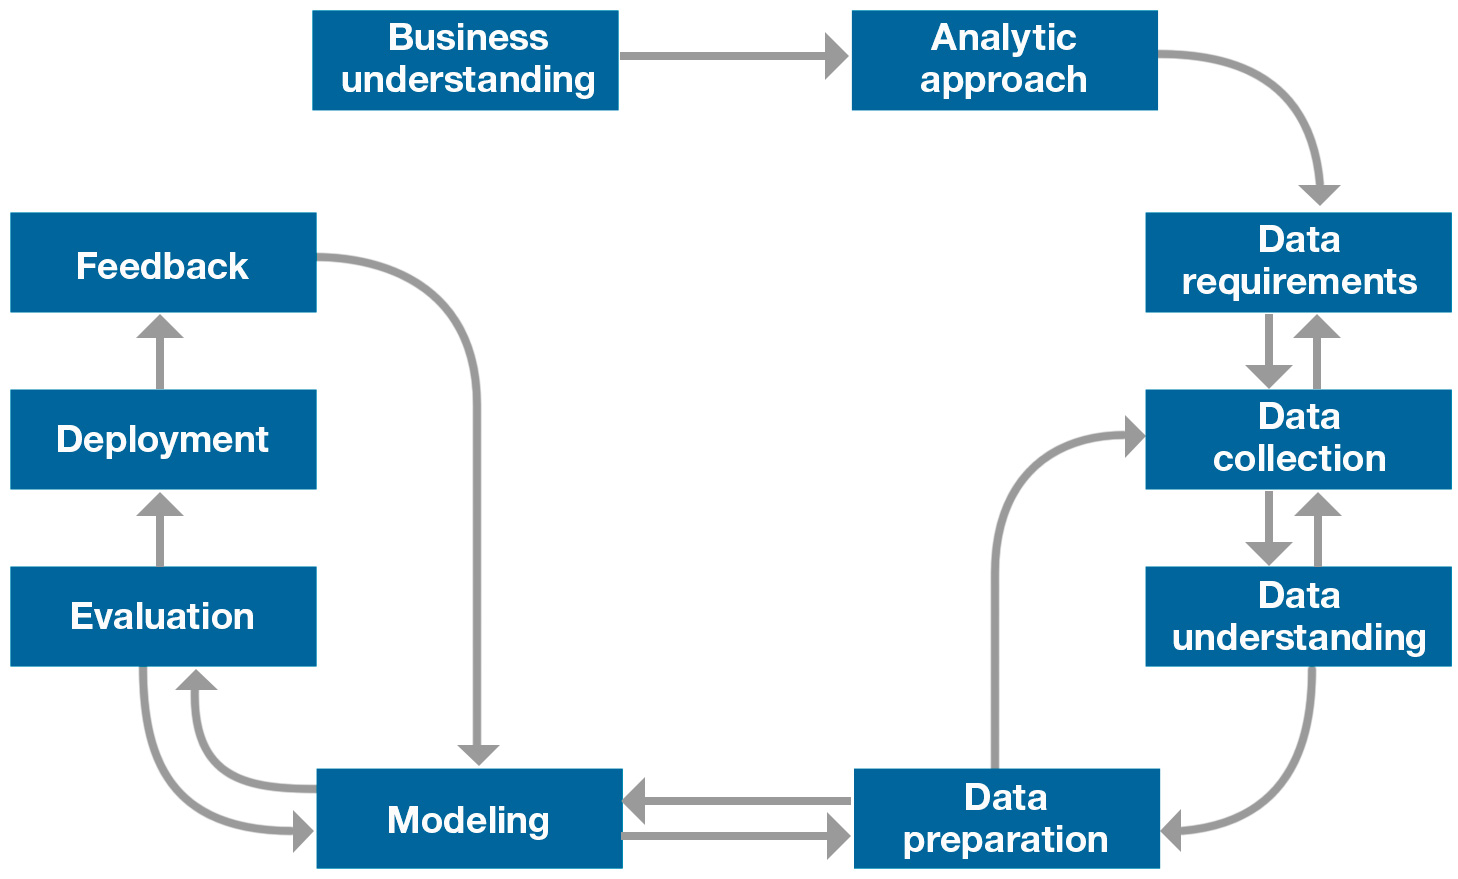
\includegraphics[width=\linewidth]{chapter1/figure/methodology.jpg}
	\caption{Foundational Methodology for Data Science by IBM \url{https://www-01.ibm.com/common/ssi/cgi-bin/ssialias?htmlfid=IMW14824USEN}}
	\label{fig:methodology}
\end{figure}

The thesis follows the typical steps of the Data Science methodology outlined in Figure \ref{fig:methodology} and makes the following \textbf{contributions}:

\begin{itemize}
	\item[\PencilRight] We construct and share \emph{four labeled datasets} containing NSFW, News-Spreaders, Spam-Bots and Fake-Followers accounts in Twitter.
	
	\item[\PencilRight] We train and study different \emph{classification algorithms}	for the categorization of accounts into the five classes of harm identified by our dataset.
	
	\item[\PencilRight] We compare the \emph{performance} (precision, recall, f-measure) of the methods against that of a baseline classifier that uses only simple profile data for classification and demonstrate the \emph{viability} of the approach.
	
	\item[\PencilRight] We compare different \emph{ensemble methods} in order to combine the best classifiers and compute  the final predictions over users.
	
	\item[\PencilRight] We describe two \emph{applications} of the best method: an implementation of a harmful bot detection tool, BotBuster, whose performance we compare with that of our reference state-of-the-art tool, i.e., Botometer (\url{https://botometer.iuni.iu.edu}); and an estimation of the global bot ecosystem of Twitter, starting from a random sampling of 12616 accounts.
	
	\item[\PencilRight] BotBuster is accessible for free at \url{http://botbuster.it} for testing.
\end{itemize}


\section{Structure of Thesis}

The thesis has the following structure:

\begin{itemize}
\item[\PencilRight] Chapter 2 introduces the state of the art.

\item[\PencilRight] Chapter 3 explores existing datasets and tools for data collection. Then it shows how the data were gathered and it ends with the \emph{creation of our datasets}.

\item[\PencilRight] Chapter 4 explains the features engineering step. Here we create new features based on users and tweets, that allow the classifiers to better understand the users' behaviours. At the end of this chapter we will have two \emph{feature vectors}: one for the binary problem (bot-or-not) and one for the multi-class problem.

\item[\PencilRight] Chapter 5 compares different classifiers for both the \emph{binary} and the \emph{multi-class} problems and performs the tuning of the parameters. In the end we will have three bot-behaviour-specific classifiers and a bot-or-not classifier.

\item[\PencilRight] Chapter 6 identifies the best way to combine the three multi-class classifiers and performs the tuning of the ensemble parameters. Then it explains the final \emph{prediction pipeline} that, starting from a user ID, returns the probabilities of membership for each class (bot, genuine) and bots sub-class (NSFW, News-Spreaders, Spam-Bots, Fake-Followers).

\item[\PencilRight] Chapter 7 describes the development of the \emph{web application (BotBuster)}. This tool provides the account classification service, according to the \emph{prediction pipeline}.

\item[\PencilRight] Chapter 8 draws conclusions, examines possible future works and estimates the global distribution of users on Twitter, by classifying randomly sampled users with our tool.


\end{itemize}

